\documentclass[border=20pt]{standalone}
\renewcommand\familydefault{\sfdefault} % Default family: serif 
%\usepackage[usenames,dvipsnames]{xcolor}
\usepackage[x11names]{xcolor}
\usepackage{tikz}
\usepackage{soulutf8}
\usetikzlibrary{arrows,fit,positioning,shapes,calc}

%\definecolor{WIRE}{HTML}{002FA7} % Klein Blue
\usepackage[normalem]{ulem}

\tikzstyle{every entity} = []
\tikzstyle{every weak entity} = []
\tikzstyle{every attribute} = []
\tikzstyle{every relationship} = []
\tikzstyle{every link} = []
\tikzstyle{every isa} = []

\tikzstyle{link} = [>=triangle 60, draw, thick, every link]

\tikzstyle{total} = [link, double, double distance=3pt]

\tikzstyle{entity} = [rectangle, draw, black, very thick,
minimum width=6em, minimum height=3em,
every entity]

\tikzstyle{weak entity} = [entity, double, double distance=2pt,
every weak entity]

\tikzstyle{attribute} = [ellipse, draw, black, very thick,
minimum width=5em, minimum height=2em,
every attribute]

%\tikzstyle{key attribute} = [attribute, font=\bfseries]

\tikzstyle{multi attribute} = [attribute, double, double distance=2pt]

\tikzstyle{derived attribute} = [attribute, dashed]

%\tikzstyle{discriminator} = [attribute, font=\itshape]

\tikzstyle{relationship} = [diamond, draw, black, very thick,
minimum width=2em, aspect=1,
every relationship]

\tikzstyle{ident relationship} = [relationship, double, double distance=2pt]

\tikzstyle{isa} = [isosceles triangle, isosceles triangle apex angle=60,
shape border rotate=-90,
draw, black, very thick, minimum size=3em,
every isa]

% for text un key attributes
\newcommand{\key}[1]{\underline{#1}}
\newcommand{\pkey}[1]{\dashuline{#1}}

% for text in discriminator attributes
\def\discriminator{\bgroup 
	\ifdim\ULdepth=\maxdimen  % Set depth based on font, if not set already
	\settodepth\ULdepth{(j}\advance\ULdepth.4pt\fi
	\markoverwith{\kern.15em
		\vtop{\kern\ULdepth \hrule width .3em}%
		\kern.15em}\ULon}

%%


\definecolor{MediumPurple1}{rgb}{0.58, 0.44, 0.86}
\definecolor{Chartreuse2}{rgb}{0.5, 1.0, 0.0}
\tikzset{every entity/.style={draw=orange, fill=orange!20}}
\tikzset{every attribute/.style={draw=MediumPurple1, fill=MediumPurple1!20}}
\tikzset{every relationship/.style={draw=Chartreuse2, fill=Chartreuse2!20}}

%% Variable for participation constraint
\newcommand{\cM}{\mathrm{M}}
\newcommand{\cN}{\mathrm{N}}
\newcommand{\cO}{\mathrm{O}}
\newcommand{\cP}{\mathrm{P}}

\begin{document}


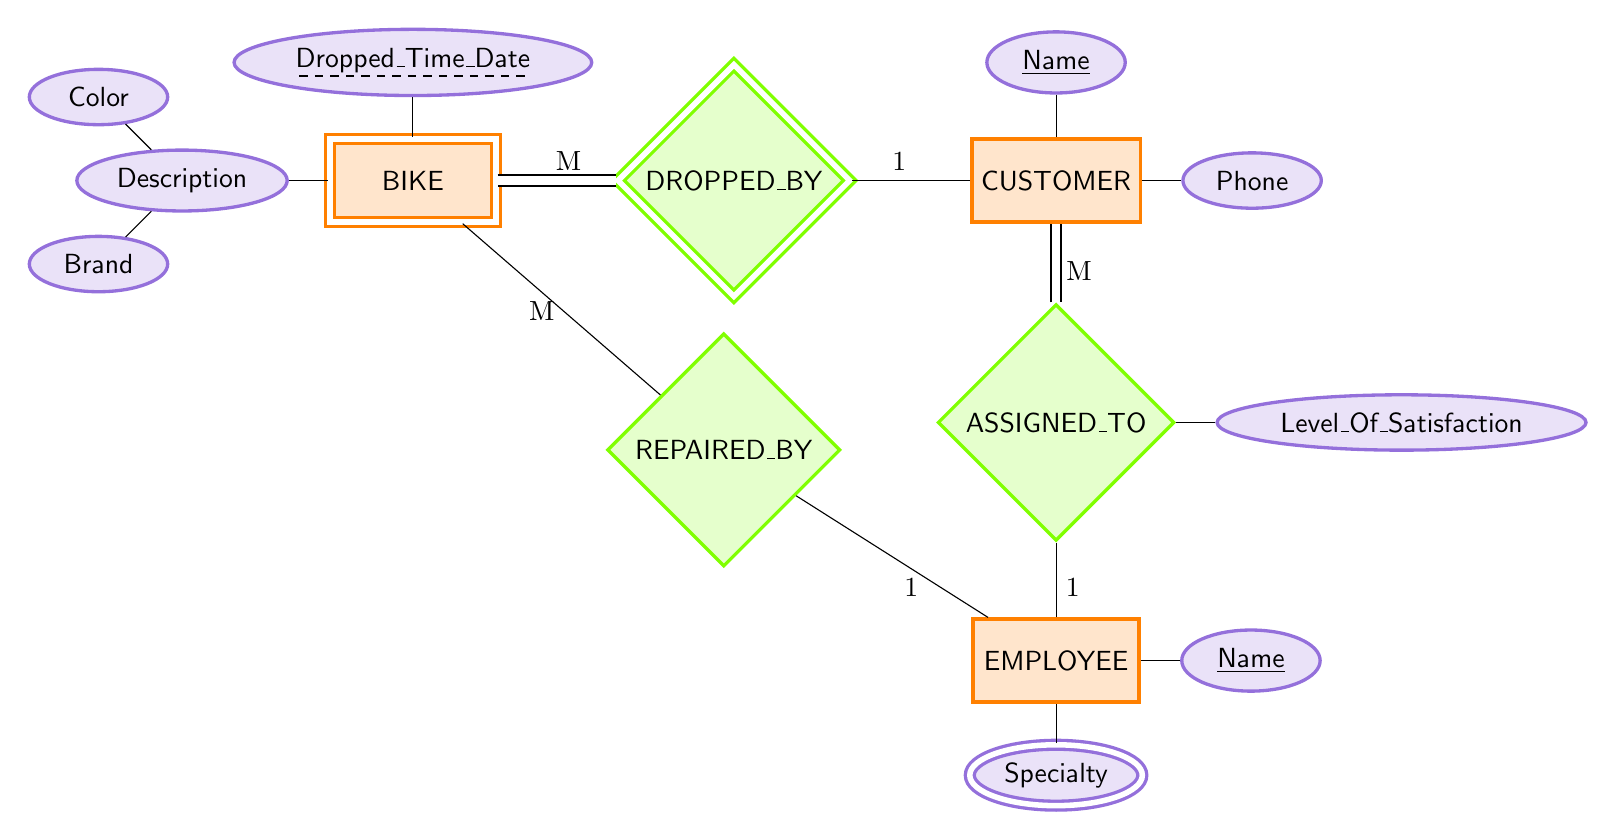
\begin{tikzpicture}[node distance=1.5cm]
	\node[entity] (CUSTOMER) {CUSTOMER};
	\node[attribute] [above of=CUSTOMER] {\key{Name}} edge (CUSTOMER);
	\node[attribute] [right = .5cm of CUSTOMER] {Phone} edge (CUSTOMER);
	%
	\node[ident relationship] (DROPPEDBY) [left = 1.5cm of CUSTOMER] {DROPPED\_BY} edge node[above, pos=0.4] {$1$} (CUSTOMER);
	%
	\node[weak entity] (BIKE) [left = 1.5cm of DROPPEDBY] {BIKE} edge[total] node[above, pos=0.6]{$\cM$} (DROPPEDBY);
	\node[attribute] [above of = BIKE] {\pkey{Dropped\_Time\_Date}} edge (BIKE);
	\node[attribute] (Description) [left = 0.5cm of BIKE] {Description} edge (BIKE);
	\node[attribute] [above left of = Description] {Color} edge (Description);
	\node[attribute] [below left of = Description] {Brand} edge (Description);
	%
	\node[relationship] (ASSIGNEDTO) [below =1cm of CUSTOMER] {ASSIGNED\_TO} edge [total] node[right, pos=0.4] {$\cM$} (CUSTOMER);
	\node[attribute] [right = .5cm of ASSIGNEDTO] {Level\_Of\_Satisfaction} edge (ASSIGNEDTO);
	%
	\node[entity] (EMPLOYEE) [below = 5cm of CUSTOMER] {EMPLOYEE} edge node[right, pos=0.4] {$1$} (ASSIGNEDTO);
	\node[attribute] [right = .5cm of EMPLOYEE] {\key{Name}} edge (EMPLOYEE);
	\node[multi attribute] [below = .5cm of EMPLOYEE] {Specialty} edge (EMPLOYEE);
	%
	\node[relationship] (REPAIREDBY) [below right =3cm of BIKE] {REPAIRED\_BY} edge node[below, pos=0.6] {$\cM$} (BIKE) edge node[below, pos=0.6] {$1$} (EMPLOYEE);

	
%\node[entity] (CUSTOMER) {CUSTOMER};
%
%
%
%\node[relationship] (SPEAKS) [below right of=CUSTOMER] {SPEAKS} edge node[right, pos=0.4] {$M$} (CUSTOMER);
%\node[entity] (LANGUAGE) [below right of=SPEAKS] {LANGUAGE} edge node[right, pos=0.5] {$N$} (SPEAKS);
%\node[attribute] (code) [left of = LANGUAGE] {\key{Code}} edge (LANGUAGE);
%\node[attribute] (symbol) [right of = LANGUAGE] {Name} edge (LANGUAGE);
%
%\node[relationship] (BWF) [below of = LANGUAGE] {B\_W\_F};
%\draw (LANGUAGE) to node[left, pos=0.6] {$N$} (BWF.west);
%\draw (LANGUAGE) to node[right, pos=0.6] {$M$} (BWF.east);
%
%
%\node[multi attribute] (color) [right =1cm of anthem] {Creator} edge (anthem);

%
%\node[relationship] (WIN) [above right of =LANGUAGE] {W\_IN};
%\draw (LANGUAGE) to node[left, pos=0.6] {$N$} (WIN);
%\draw (anthem) to node[right, pos=0.6] {$M$} (WIN);

\end{tikzpicture}

\end{document}
